\documentclass{article}

\usepackage[margin=1in]{geometry} % Set margins to 1 inch
\usepackage{graphicx} % Allows including images
\usepackage{float} % Allows for precise placement of figures
\usepackage{amsmath} % Allows for math equations
\usepackage{siunitx} % Allows for SI units
\usepackage{placeins} % Makes sure images are in their respective sections by \FloatBarrier

\begin{document}

\title{Software Assignment Report\\ \large{Aditya Gawande\\EE22BTECH11202}}
\author{}
\date{}
\maketitle

\maketitle

\section*{Aim}
Aim of this assignment is to make a python script which can make a playlist of songs and shuffle them. The songs must be shuffled such that each song in the playlist is played before it gets looped.

\section{Overview}
\begin{itemize}
    \item Use of numpy library is allowed to randomize playlist.
    \item The songs must be played through either terminal or GUI.
    \item Tkintker library has been used in the program to make the window.
    \item PyGame library has been used to play audio files.
    \item os module has been used to search file directory (cwd/songs) by default.
\end{itemize}

\begin{figure}[ht]
	\centering
	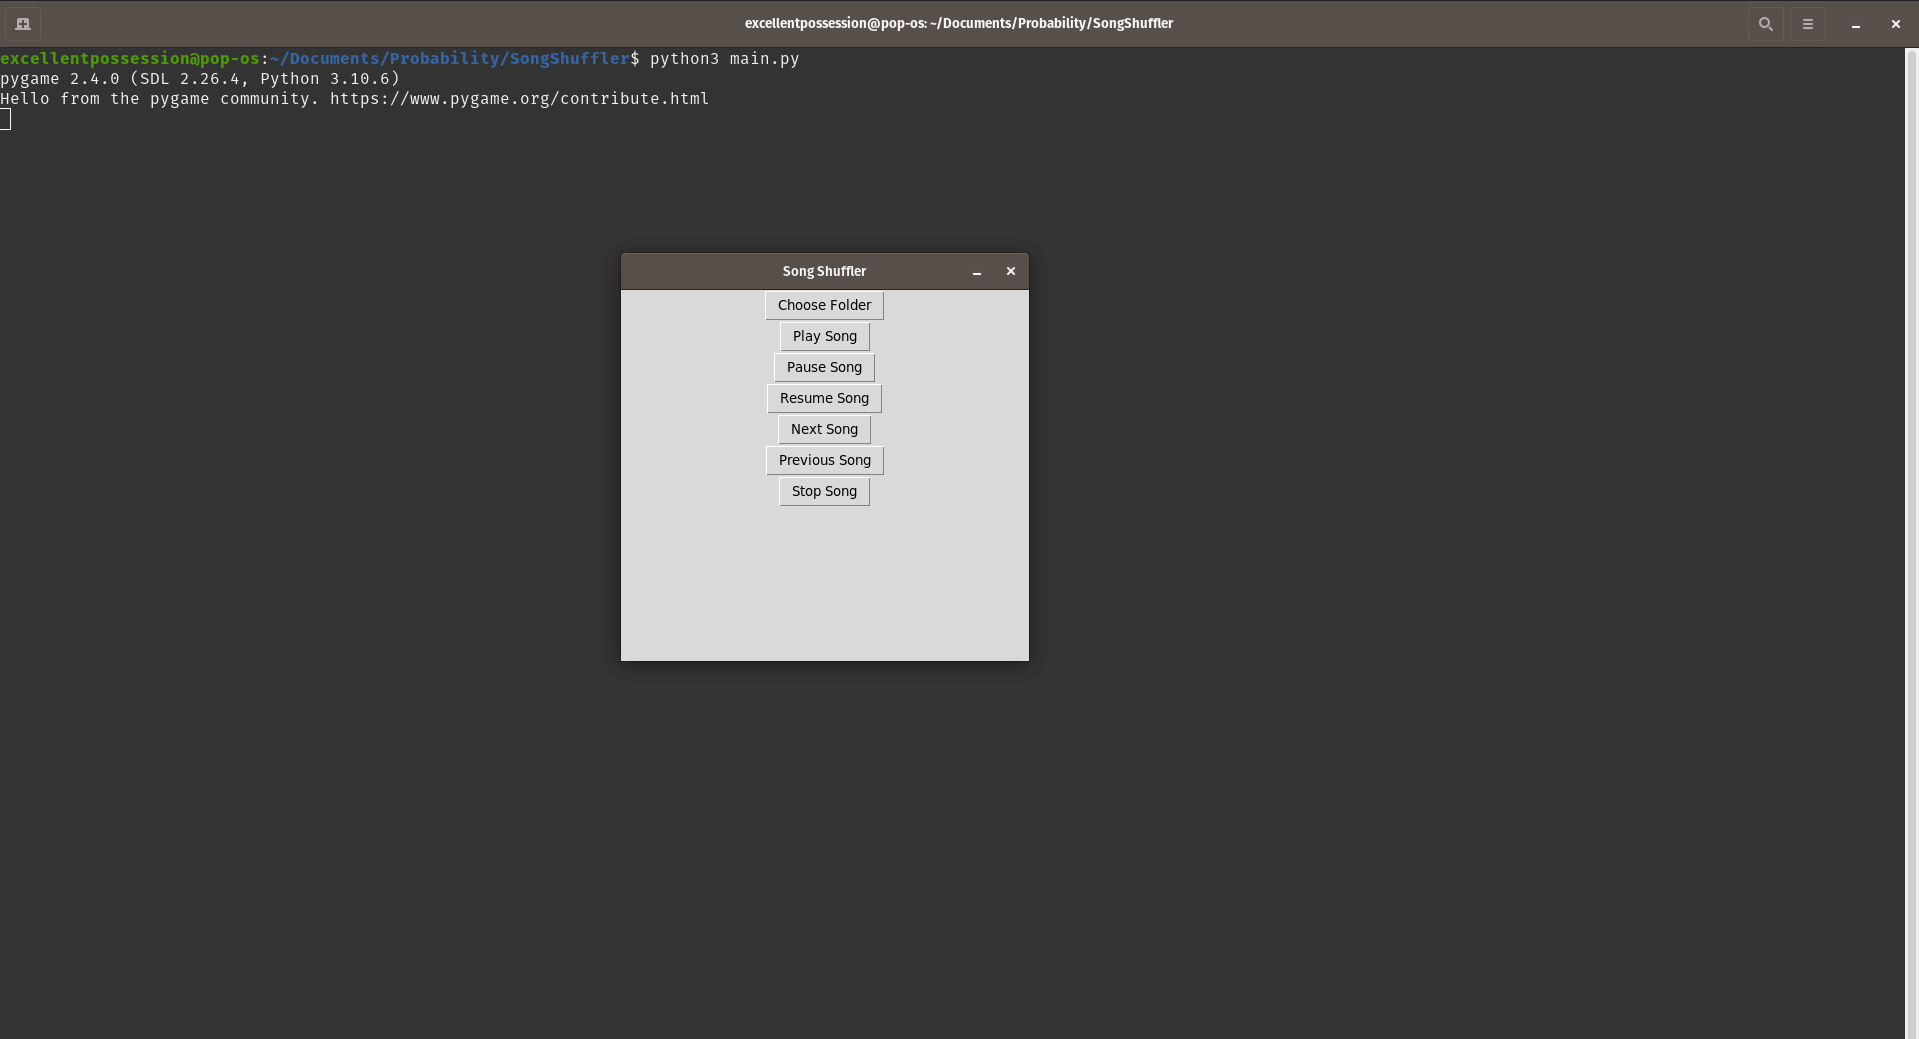
\includegraphics[width=0.7\linewidth]{figs/UI.png}
	\caption{Screenshot of the UI}
	\label{fig:view}
\end{figure}
\FloatBarrier


\section{Working}
\begin{enumerate}
    \item The program scans the default folder and makes a list of all the mp3 files present in it.
    \item shuffle function in the program randomizes the order of the music files.
    \item Because the function only randomizes the order, there is no repetition of songs in the playlist, which is one of the conditions of the assignment.
    \item File managing is done completely through os module functions.
    \item Audio file playback is handled entirely through PyGame module functions. (Pygame mixer is used)
\end{enumerate}
\subsection*{Shuffle function}
\begin{enumerate}
    \item It replaces two elements with the second element to be replaced taken from randint function of numpy.random.
    \item As it replaces the elements, there is no repetition in the playlist.
    \item This function is executed whenever the playlist reaches the last song and user presses next song button.
\end{enumerate}

\section{Notes}
\begin{itemize}
    \item All of this code can easily be converted into a terminal script, as the functions are not part of the tkinter library.
    \item The program can be used to play mp3 present in any directory, and it has a button to select directories too.
    \item This can be used to play different file formats in a shuffled way, if the playback functions are changed accordingly.
\end{itemize}

 



\end{document}
